
\section{Results}
\label{sec:results}

\begin{table*}[ht]
  \centering
  \begin{tabular}{|c|c|}
    \hline \hline % draws two horizontal lines at the top of the table
    Algorithm & Margin of Victory\\
    \hline % line after the column headers
    M1& $-777.8$\\
    M2& $-893.7$\\
    M3& $-1082.4$\\
    M4& $-1521.0$\\
    M5& $-1821.6$\\
    M6& $-2702.4$\\
    \hline
    H1& $-2147.3$\\
    H2& $-2859.9$\\
    \hline
    F1& $285.8$\\
    F2& $271.8$\\
    \hline
    S1& $9.7$\\
    S2& $0.9$\\
    S3& $-251.1$\\
    \hline
    L1& $31.9$\\
    \hline
    G1& $35.7$\\
    \hline \hline
  \end{tabular}
  
  \caption{Regret-minimization algorithm margin of victory against other algorithms.}
  \label{tab:data}
\end{table*}

The results of the competition can be seen in Table~\ref{tab:data}.  Meta-strategy algorithms are labelled with M's, historical prediction with H's, frequency analysis with F's, static mixed strategies with S's, the reinforcement learning with an L, and the gambit technique with a G.  Note that negative margins of victory indicate that our algorithm was, on average, less successful than the opponent algorithm, and that small average margins of victory (below $100$) indicate that the algorithms primarily tie against each other, and would likely average out in the long term.

Overall, it's quite clear from the data that this algorithm is not particularly competitive in Rock-Paper-Scissors.  It loses rather spectacularly to the meta-strategy algorithms and to the historical prediction algorithms.  While the regret minimization algorithm does typically beat frequency analysis algorithms, the victory is by a relatively small margin.  

We suspect that the historical prediction algorithms perform so strongly against the regret minimization algorithm because our algorithm is prone to sequences of repeated action choice when it identifies a sizable regret in the recent past.  The historical prediction algorithms likely identify such sequences quickly and react accordingly, as a sequence of identical plays need not be particularly long before a historical prediction algorithm is simply attempting to match a those identical plays.

The performance of meta-strategy algorithms against our algorithm is unsurprising, as such algorithms are employed by the most successful algorithms in public competitions \cite{rpscomp}.  Such meta-algorithms, which  choose the anticipated best algorithm from amongst a set of candidates, are extremely versatile.

Of curious note is the regret minimization algorithm's performance against the static mixed-strategy algorithms.  The original regret minimization technique from which our algorithm is derived was intended for use as an approach for beating static mixed strategies.  The altered algorithm no longer out-competes such algorithms, instead tying or losing.  We suspect that the alterations we have made, needed to adapt to non-static strategies, have compromised the algorithm's performance against true static mixed strategies.  In particular, in exploring a limited depth of recent history to build a current regret prediction, the algorithm may be susceptible to short-term trends in opponent performance which, while meaningful against adaptive and logical opponents, limits the algorithm's accuracy against static mixed strategy algorithms by encouraging more erratic behavior \cite{noregrets}.  

%Present the results of your experiments. Simply presenting the data is
%insufficient! You need to analyze your results. What did you discover?
%What is interesting about your results? Were the results what you
%expected? Use appropriate visualizations. Prefer graphs and charts to
%tables as they are easier to read (though tables are often more
%compact, and can be a better choice if you're squeezed for space).
%\textbf{Always} include information that conveys the uncertainty in
%your measurements: mean statistics should be plotted with error bars,
%or reported in tables with a $\pm$ range. The $95\%$-confidence
%interval is a commonly reported statistic.

%\subsection{Embedding Pictures}
%\label{subsec:pics}

%See the source code (\texttt{results.tex}) for instructions on how to
%insert figures (like figure~\ref{fig:tex}) or plots into your
%document.

% Note that TeX has a mind of its own when it comes to placing images
% in documents - where a figure appears in the PDF document will often
% be quite different from where it appears in the source code. This is
% a feature, not a bug - it enables LaTeX to produce layouts that
% "flow" better. It only takes a few lines to insert a figure into
% your write-up - I recommend using PNG, JPG or PDF images
% (incidentally, programs like Excel and Matlab will allow you to save
% any plots or figures you generate in those formats). The \figure{}
% command is used to create a new figure.
%\begin{figure}[htb]

%  \centering  % centers the image in the column

  % replace the second argument below with your filename. I like to
  % place all my figures in a sub-directory to keep things organized
%  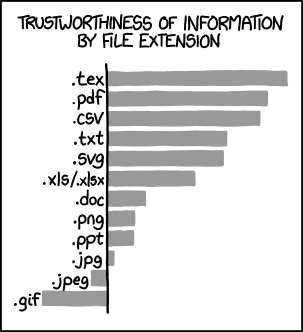
\includegraphics[width=0.47\textwidth]{figs/file_extensions.png}

  % *Every* figure should have a descriptive caption.
%  \caption{On the trustworthiness of \LaTeX. Image courtesy of \texttt{xkcd}.}

  % The label is a handle you create so that you can refer to this
  % figure (using the \ref{} command) from other parts of your
  % document. LaTeX automatically renumbers figures and updates
  % references when you recompile, so you should do it this way rather
  % than hard-coding in references. Notice that I've also been
  % creating labels for the various sections in the document; I could
  % use \ref{} command to refer to those sections using their labels
  % too.
  %\label{fig:tex}

%\end{figure}

%\subsection{Creating Tables}
%\label{subsec:tables}

%Again, refer to \texttt{results.tex} to learn how to create simple
%tables (like table~\ref{tab:example}).


